\section{Sets and Relations}

\begin{definition}[Polyhedral Set]
A {\em polyhedral set}\index{polyhedral set} $S$ is a finite union of basic sets
$S = \bigcup_i S_i$, each of which can be represented using affine
constraints
$$
S_i : \Z^n \to 2^{\Z^d} : \vec s \mapsto
S_i(\vec s) =
\{\, \vec x \in \Z^d \mid \exists \vec z \in \Z^e :
A \vec x + B \vec s + D \vec z + \vec c \geq \vec 0 \,\}
,
$$
with $A \in \Z^{m \times d}$,
$B \in \Z^{m \times n}$,
$D \in \Z^{m \times e}$
and $\vec c \in \Z^m$.
\end{definition}

\begin{definition}[Parameter Domain of a Set]
Let $S \in \Z^n \to 2^{\Z^d}$ be a set.
The {\em parameter domain} of $S$ is the set
$$\pdom S \coloneqq \{\, \vec s \in \Z^n \mid S(\vec s) \ne \emptyset \,\}.$$
\end{definition}

\begin{definition}[Polyhedral Relation]
A {\em polyhedral relation}\index{polyhedral relation}
$R$ is a finite union of basic relations
$R = \bigcup_i R_i$ of type
$\Z^n \to 2^{\Z^{d_1+d_2}}$,
each of which can be represented using affine
constraints
$$
R_i = \vec s \mapsto
R_i(\vec s) =
\{\, \vec x_1 \to \vec x_2 \in \Z^{d_1} \times \Z^{d_2}
\mid \exists \vec z \in \Z^e :
A_1 \vec x_1 + A_2 \vec x_2 + B \vec s + D \vec z + \vec c \geq \vec 0 \,\}
,
$$
with $A_i \in \Z^{m \times d_i}$,
$B \in \Z^{m \times n}$,
$D \in \Z^{m \times e}$
and $\vec c \in \Z^m$.
\end{definition}

\begin{definition}[Parameter Domain of a Relation]
Let $R \in \Z^n \to 2^{\Z^{d+d}}$ be a relation.
The {\em parameter domain} of $R$ is the set
$$\pdom R \coloneqq \{\, \vec s \in \Z^n \mid R(\vec s) \ne \emptyset \,\}.$$
\end{definition}

\begin{definition}[Domain of a Relation]
Let $R \in \Z^n \to 2^{\Z^{d+d}}$ be a relation.
The {\em domain} of $R$ is the polyhedral set
$$\domain R \coloneqq \vec s \mapsto
\{\, \vec x_1 \in \Z^{d_1} \mid \exists \vec x_2 \in \Z^{d_2} :
(\vec x_1, \vec x_2) \in R(\vec s) \,\}
.
$$
\end{definition}

\begin{definition}[Range of a Relation]
Let $R \in \Z^n \to 2^{\Z^{d+d}}$ be a relation.
The {\em range} of $R$ is the polyhedral set
$$
\range R \coloneqq \vec s \mapsto
\{\, \vec x_2 \in \Z^{d_2} \mid \exists \vec x_1 \in \Z^{d_1} :
(\vec x_1, \vec x_2) \in R(\vec s) \,\}
.
$$
\end{definition}

\begin{definition}[Composition of Relations]
Let $R \in \Z^n \to 2^{\Z^{d_1+d_2}}$ and
$S \in \Z^n \to 2^{\Z^{d_2+d_3}}$ be two relations,
then the composition of
$R$ and $S$ is defined as
$$
S \circ R \coloneqq
\vec s \mapsto
\{\, \vec x_1 \to \vec x_3 \in \Z^{d_1} \times \Z^{d_3}
\mid \exists \vec x_2 \in \Z^{d_2} :
\vec x_1 \to \vec x_2 \in R(\vec s) \wedge
\vec x_2 \to \vec x_3 \in S(\vec s)
\,\}
.
$$
\end{definition}

\begin{definition}[Difference Set of a Relation]
Let $R \in \Z^n \to 2^{\Z^{d+d}}$ be a relation.
The difference set ($\Delta \, R$) of $R$ is the set
of differences between image elements and the corresponding
domain elements,
$$
\diff R \coloneqq
\vec s \mapsto
\{\, \vec \delta \in \Z^{d} \mid \exists \vec x \to \vec y \in R :
\vec \delta = \vec y - \vec x
\,\}
$$
\end{definition}

\section{Simple Hull}\label{s:simple hull}

It is sometimes useful to have a single
basic set or basic relation that contains a given set or relation.
For rational sets, the obvious choice would be to compute the
(rational) convex hull.  For integer sets, the obvious choice
would be the integer hull.
However, {\tt isl} currently does not support an integer hull operation
and even if it did, it would be fairly expensive to compute.
The convex hull operation is supported, but it is also fairly
expensive to compute given only an implicit representation.

Usually, it is not required to compute the exact integer hull,
and an overapproximation of this hull is sufficient.
The ``simple hull'' of a set is such an overapproximation
and it is defined as the (inclusion-wise) smallest basic set
that is described by constraints that are translates of
the constraints in the input set.
This means that the simple hull is relatively cheap to compute
and that the number of constraints in the simple hull is no
larger than the number of constraints in the input.
\begin{definition}[Simple Hull of a Set]
The {\em simple hull} of a set
$S = \bigcup_{1 \le i \le v} S_i$, with
$$
S : \Z^n \to 2^{\Z^d} : \vec s \mapsto
S(\vec s) =
\left\{\, \vec x \in \Z^d \mid \exists \vec z \in \Z^e :
\bigvee_{1 \le i \le v}
A_i \vec x + B_i \vec s + D_i \vec z + \vec c_i \geq \vec 0 \,\right\}
$$
is the set
$$
H : \Z^n \to 2^{\Z^d} : \vec s \mapsto
S(\vec s) =
\left\{\, \vec x \in \Z^d \mid \exists \vec z \in \Z^e :
\bigwedge_{1 \le i \le v}
A_i \vec x + B_i \vec s + D_i \vec z + \vec c_i + \vec K_i \geq \vec 0
\,\right\}
,
$$
with $\vec K_i$ the (component-wise) smallest non-negative integer vectors
such that $S \subseteq H$.
\end{definition}
The $\vec K_i$ can be obtained by solving a number of
LP problems, one for each element of each $\vec K_i$.
If any LP problem is unbounded, then the corresponding constraint
is dropped.

\section{Parametric Integer Programming}

\subsection{Introduction}\label{s:intro}

Parametric integer programming \shortcite{Feautrier88parametric}
is used to solve many problems within the context of the polyhedral model.
Here, we are mainly interested in dependence analysis \shortcite{Fea91}
and in computing a unique representation for existentially quantified
variables.  The latter operation has been used for counting elements
in sets involving such variables
\shortcite{BouletRe98,Verdoolaege2005experiences} and lies at the core
of the internal representation of {\tt isl}.

Parametric integer programming was first implemented in \texttt{PipLib}.
An alternative method for parametric integer programming
was later implemented in {\tt barvinok} \cite{barvinok-0.22}.
This method is not based on Feautrier's algorithm, but on rational
generating functions \cite{Woods2003short} and was inspired by the
``digging'' technique of \shortciteN{DeLoera2004Three} for solving
non-parametric integer programming problems.

In the following sections, we briefly recall the dual simplex
method combined with Gomory cuts and describe some extensions
and optimizations.  The main algorithm is applied to a matrix
data structure known as a tableau.  In case of parametric problems,
there are two tableaus, one for the main problem and one for
the constraints on the parameters, known as the context tableau.
The handling of the context tableau is described in \autoref{s:context}.

\subsection{The Dual Simplex Method}

Tableaus can be represented in several slightly different ways.
In {\tt isl}, the dual simplex method uses the same representation
as that used by its incremental LP solver based on the \emph{primal}
simplex method.  The implementation of this LP solver is based
on that of {\tt Simplify} \shortcite{Detlefs2005simplify}, which, in turn,
was derived from the work of \shortciteN{Nelson1980phd}.
In the original \shortcite{Nelson1980phd}, the tableau was implemented
as a sparse matrix, but neither {\tt Simplify} nor the current
implementation of {\tt isl} does so.

Given some affine constraints on the variables,
$A \vec x + \vec b \ge \vec 0$, the tableau represents the relationship
between the variables $\vec x$ and non-negative variables
$\vec y = A \vec x + \vec b$ corresponding to the constraints.
The initial tableau contains $\begin{pmatrix}
\vec b & A
\end{pmatrix}$ and expresses the constraints $\vec y$ in the rows in terms
of the variables $\vec x$ in the columns.  The main operation defined
on a tableau exchanges a column and a row variable and is called a pivot.
During this process, some coefficients may become rational.
As in the \texttt{PipLib} implementation,
{\tt isl} maintains a shared denominator per row.
The sample value of a tableau is one where each column variable is assigned
zero and each row variable is assigned the constant term of the row.
This sample value represents a valid solution if each constraint variable
is assigned a non-negative value, i.e., if the constant terms of
rows corresponding to constraints are all non-negative.

The dual simplex method starts from an initial sample value that
may be invalid, but that is known to be (lexicographically) no
greater than any solution, and gradually increments this sample value
through pivoting until a valid solution is obtained.
In particular, each pivot exchanges a row variable
$r = -n + \sum_i a_i \, c_i$ with negative
sample value $-n$ with a column variable $c_j$
such that $a_j > 0$.  Since $c_j = (n + r - \sum_{i\ne j} a_i \, c_i)/a_j$,
the new row variable will have a positive sample value $n$.
If no such column can be found, then the problem is infeasible.
By always choosing the column that leads to the (lexicographically)
smallest increment in the variables $\vec x$,
the first solution found is guaranteed to be the (lexicographically)
minimal solution \cite{Feautrier88parametric}.
In order to be able to determine the smallest increment, the tableau
is (implicitly) extended with extra rows defining the original
variables in terms of the column variables.
If we assume that all variables are non-negative, then we know
that the zero vector is no greater than the minimal solution and
then the initial extended tableau looks as follows.
$$
\begin{tikzpicture}
\matrix (m) [matrix of math nodes]
{
& {} & 1 & \vec c \\
\vec x && |(top)| \vec 0 & I \\
\vec r && \vec b & |(bottom)|A \\
};
\begin{pgfonlayer}{background}
\node (core) [inner sep=0pt,fill=black!20,right delimiter=),left delimiter=(,fit=(top)(bottom)] {};
\end{pgfonlayer}
\end{tikzpicture}
$$
Each column in this extended tableau is lexicographically positive
and will remain so because of the column choice explained above.
It is then clear that the value of $\vec x$ will increase in each step.
Note that there is no need to store the extra rows explicitly.
If a given $x_i$ is a column variable, then the corresponding row
is the unit vector $e_i$.  If, on the other hand, it is a row variable,
then the row already appears somewhere else in the tableau.

In case of parametric problems, the sign of the constant term
may depend on the parameters.  Each time the constant term of a constraint row
changes, we therefore need to check whether the new term can attain
negative and/or positive values over the current set of possible
parameter values, i.e., the context.
If all these terms can only attain non-negative values, the current
state of the tableau represents a solution.  If one of the terms
can only attain non-positive values and is not identically zero,
the corresponding row can be pivoted.
Otherwise, we pick one of the terms that can attain both positive
and negative values and split the context into a part where
it only attains non-negative values and a part where it only attains
negative values.

\subsection{Gomory Cuts}

The solution found by the dual simplex method may have
non-integral coordinates.  If so, some rational solutions
(including the current sample value), can be cut off by
applying a (parametric) Gomory cut.
Let $r = b(\vec p) + \sp {\vec a} {\vec c}$ be the row
corresponding to the first non-integral coordinate of $\vec x$,
with $b(\vec p)$ the constant term, an affine expression in the
parameters $\vec p$, i.e., $b(\vec p) = \sp {\vec f} {\vec p} + g$.
Note that only row variables can attain
non-integral values as the sample value of the column variables is zero.
Consider the expression
$b(\vec p) - \ceil{b(\vec p)} + \sp {\fract{\vec a}} {\vec c}$,
with $\ceil\cdot$ the ceiling function and $\fract\cdot$ the
fractional part.  This expression is negative at the sample value
since $\vec c = \vec 0$ and $r = b(\vec p)$ is fractional, i.e.,
$\ceil{b(\vec p)} > b(\vec p)$.  On the other hand, for each integral
value of $r$ and $\vec c \ge 0$, the expression is non-negative
because $b(\vec p) - \ceil{b(\vec p)} > -1$.
Imposing this expression to be non-negative therefore does not
invalidate any integral solutions, while it does cut away the current
fractional sample value.  To be able to formulate this constraint,
a new variable $q = \floor{-b(\vec p)} = - \ceil{b(\vec p)}$ is added
to the context.  This integral variable is uniquely defined by the constraints
$0 \le -d \, b(\vec p) - d \, q \le d - 1$, with $d$ the common
denominator of $\vec f$ and $g$.  In practice, the variable
$q' = \floor{\sp {\fract{-f}} {\vec p} + \fract{-g}}$ is used instead
and the coefficients of the new constraint are adjusted accordingly.
The sign of the constant term of this new constraint need not be determined
as it is non-positive by construction.
When several of these extra context variables are added, it is important
to avoid adding duplicates.
Recent versions of {\tt PipLib} also check for such duplicates.

\subsection{Negative Unknowns and Maximization}

There are two places in the above algorithm where the unknowns $\vec x$
are assumed to be non-negative: the initial tableau starts from
sample value $\vec x = \vec 0$ and $\vec c$ is assumed to be non-negative
during the construction of Gomory cuts.
To deal with negative unknowns, \shortciteN[Appendix A.2]{Fea91}
proposed to use a ``big parameter'', say $M$, that is taken to be
an arbitrarily large positive number.  Instead of looking for the
lexicographically minimal value of $\vec x$, we search instead
for the lexicographically minimal value of $\vec x' = \vec M + \vec x$.
The sample value $\vec x' = \vec 0$ of the initial tableau then
corresponds to $\vec x = -\vec M$, which is clearly not greater than
any potential solution.  The sign of the constant term of a row
is determined lexicographically, with the coefficient of $M$ considered
first.  That is, if the coefficient of $M$ is not zero, then its sign
is the sign of the entire term.  Otherwise, the sign is determined
by the remaining affine expression in the parameters.
If the original problem has a bounded optimum, then the final sample
value will be of the form $\vec M + \vec v$ and the optimal value
of the original problem is then $\vec v$.
Maximization problems can be handled in a similar way by computing
the minimum of $\vec M - \vec x$.

When the optimum is unbounded, the optimal value computed for
the original problem will involve the big parameter.
In the original implementation of {\tt PipLib}, the big parameter could
even appear in some of the extra variables $\vec q$ created during
the application of a Gomory cut.  The final result could then contain
implicit conditions on the big parameter through conditions on such
$\vec q$ variables.  This problem was resolved in later versions
of {\tt PipLib} by taking $M$ to be divisible by any positive number.
The big parameter can then never appear in any $\vec q$ because
$\fract {\alpha M } = 0$.  It should be noted, though, that an unbounded
problem usually (but not always)
indicates an incorrect formulation of the problem.

The original version of {\tt PipLib} required the user to ``manually''
add a big parameter, perform the reformulation and interpret the result
\shortcite{Feautrier02}.  Recent versions allow the user to simply
specify that the unknowns may be negative or that the maximum should
be computed and then these transformations are performed internally.
Although there are some application, e.g.,
that of \shortciteN{Feautrier92multi},
where it is useful to have explicit control over the big parameter,
negative unknowns and maximization are by far the most common applications
of the big parameter and we believe that the user should not be bothered
with such implementation issues.
The current version of {\tt isl} therefore does not
provide any interface for specifying big parameters.  Instead, the user
can specify whether a maximum needs to be computed and no assumptions
are made on the sign of the unknowns.  Instead, the sign of the unknowns
is checked internally and a big parameter is automatically introduced when
needed.  For compatibility with {\tt PipLib}, the {\tt isl\_pip} tool
does explicitly add non-negativity constraints on the unknowns unless
the \verb+Urs_unknowns+ option is specified.
Currently, there is also no way in {\tt isl} of expressing a big
parameter in the output.  Even though
{\tt isl} makes the same divisibility assumption on the big parameter
as recent versions of {\tt PipLib}, it will therefore eventually
produce an error if the problem turns out to be unbounded.

\subsection{Preprocessing}

In this section, we describe some transformations that are
or can be applied in advance to reduce the running time
of the actual dual simplex method with Gomory cuts.

\subsubsection{Feasibility Check and Detection of Equalities}

Experience with the original {\tt PipLib} has shown that Gomory cuts
do not perform very well on problems that are (non-obviously) empty,
i.e., problems with rational solutions, but no integer solutions.
In {\tt isl}, we therefore first perform a feasibility check on
the original problem considered as a non-parametric problem
over the combined space of unknowns and parameters.
In fact, we do not simply check the feasibility, but we also
check for implicit equalities among the integer points by computing
the integer affine hull.  The algorithm used is the same as that
described in \autoref{s:GBR} below.
Computing the affine hull is fairly expensive, but it can
bring huge benefits if any equalities can be found or if the problem
turns out to be empty.

\subsubsection{Constraint Simplification}

If the coefficients of the unknown and parameters in a constraint
have a common factor, then this factor should be removed, possibly
rounding down the constant term.  For example, the constraint
$2 x - 5 \ge 0$ should be simplified to $x - 3 \ge 0$.
{\tt isl} performs such simplifications on all sets and relations.
Recent versions of {\tt PipLib} also perform this simplification
on the input.

\subsubsection{Exploiting Equalities}\label{s:equalities}

If there are any (explicit) equalities in the input description,
{\tt PipLib} converts each into a pair of inequalities.
It is also possible to write $r$ equalities as $r+1$ inequalities
\shortcite{Feautrier02}, but it is even better to \emph{exploit} the
equalities to reduce the dimensionality of the problem.
Given an equality involving at least one unknown, we pivot
the row corresponding to the equality with the column corresponding
to the last unknown with non-zero coefficient.  The new column variable
can then be removed completely because it is identically zero,
thereby reducing the dimensionality of the problem by one.
The last unknown is chosen to ensure that the columns of the initial
tableau remain lexicographically positive.  In particular, if
the equality is of the form $b + \sum_{i \le j} a_i \, x_i = 0$ with
$a_j \ne 0$, then the (implicit) top rows of the initial tableau
are changed as follows
$$
\begin{tikzpicture}
\matrix [matrix of math nodes]
{
 & {} & |(top)| 0 & I_1 & |(j)| &  \\
j && 0 & & 1 & \\
  && 0 & & & |(bottom)|I_2 \\
};
\node[overlay,above=2mm of j,anchor=south]{j};
\begin{pgfonlayer}{background}
\node (m) [inner sep=0pt,fill=black!20,right delimiter=),left delimiter=(,fit=(top)(bottom)] {};
\end{pgfonlayer}
\begin{scope}[xshift=4cm]
\matrix [matrix of math nodes]
{
 & {} & |(top)| 0 & I_1 &  \\
j && |(left)| -b/a_j & -a_i/a_j & \\
  && 0 & & |(bottom)|I_2 \\
};
\begin{pgfonlayer}{background}
\node (m2) [inner sep=0pt,fill=black!20,right delimiter=),left delimiter=(,fit=(top)(bottom)(left)] {};
\end{pgfonlayer}
\end{scope}
 \draw [shorten >=7mm,-to,thick,decorate,
        decoration={snake,amplitude=.4mm,segment length=2mm,
                    pre=moveto,pre length=5mm,post length=8mm}]
   (m) -- (m2);
\end{tikzpicture}
$$
Currently, {\tt isl} also eliminates equalities involving only parameters
in a similar way, provided at least one of the coefficients is equal to one.
The application of parameter compression (see below)
would obviate the need for removing parametric equalities.

\subsubsection{Offline Symmetry Detection}\label{s:offline}

Some problems, notably those of \shortciteN{Bygde2010licentiate},
have a collection of constraints, say
$b_i(\vec p) + \sp {\vec a} {\vec x} \ge 0$,
that only differ in their (parametric) constant terms.
These constant terms will be non-negative on different parts
of the context and this context may have to be split for each
of the constraints.  In the worst case, the basic algorithm may
have to consider all possible orderings of the constant terms.
Instead, {\tt isl} introduces a new parameter, say $u$, and
replaces the collection of constraints by the single
constraint $u + \sp {\vec a} {\vec x} \ge 0$ along with
context constraints $u \le b_i(\vec p)$.
Any solution to the new system is also a solution
to the original system since
$\sp {\vec a} {\vec x} \ge -u \ge -b_i(\vec p)$.
Conversely, $m = \min_i b_i(\vec p)$ satisfies the constraints
on $u$ and therefore extends a solution to the new system.
It can also be plugged into a new solution.
See \autoref{s:post} for how this substitution is currently performed
in {\tt isl}.
The method described in this section can only detect symmetries
that are explicitly available in the input.
See \autoref{s:online} for the detection
and exploitation of symmetries that appear during the course of
the dual simplex method.

\subsubsection{Parameter Compression}\label{s:compression}

It may in some cases be apparent from the equalities in the problem
description that there can only be a solution for a sublattice
of the parameters.  In such cases ``parameter compression''
\shortcite{Meister2004PhD,Meister2008} can be used to replace
the parameters by alternative ``dense'' parameters.
For example, if there is a constraint $2x = n$, then the system
will only have solutions for even values of $n$ and $n$ can be replaced
by $2n'$.  Similarly, the parameters $n$ and $m$ in a system with
the constraint $2n = 3m$ can be replaced by a single parameter $n'$
with $n=3n'$ and $m=2n'$.
It is also possible to perform a similar compression on the unknowns,
but it would be more complicated as the compression would have to
preserve the lexicographical order.  Moreover, due to our handling
of equalities described above there should be
no need for such variable compression.
Although parameter compression has been implemented in {\tt isl},
it is currently not yet used during parametric integer programming.

\subsection{Postprocessing}\label{s:post}

The output of {\tt PipLib} is a quast (quasi-affine selection tree).
Each internal node in this tree corresponds to a split of the context
based on a parametric constant term in the main tableau with indeterminate
sign.  Each of these nodes may introduce extra variables in the context
corresponding to integer divisions.  Each leaf of the tree prescribes
the solution in that part of the context that satisfies all the conditions
on the path leading to the leaf.
Such a quast is a very economical way of representing the solution, but
it would not be suitable as the (only) internal representation of
sets and relations in {\tt isl}.  Instead, {\tt isl} represents
the constraints of a set or relation in disjunctive normal form.
The result of a parametric integer programming problem is then also
converted to this internal representation.  Unfortunately, the conversion
to disjunctive normal form can lead to an explosion of the size
of the representation.
In some cases, this overhead would have to be paid anyway in subsequent
operations, but in other cases, especially for outside users that just
want to solve parametric integer programming problems, we would like
to avoid this overhead in future.  That is, we are planning on introducing
quasts or a related representation as one of several possible internal
representations and on allowing the output of {\tt isl\_pip} to optionally
be printed as a quast.

Currently, {\tt isl} also does not have an internal representation
for expressions such as $\min_i b_i(\vec p)$ from the offline
symmetry detection of \autoref{s:offline}.
Assume that one of these expressions has $n$ bounds $b_i(\vec p)$.
If the expression
does not appear in the affine expression describing the solution,
but only in the constraints, and if moreover, the expression
only appears with a positive coefficient, i.e.,
$\min_i b_i(\vec p) \ge f_j(\vec p)$, then each of these constraints
can simply be reduplicated $n$ times, once for each of the bounds.
Otherwise, a conversion to disjunctive normal form
leads to $n$ cases, each described as $u = b_i(\vec p)$ with constraints
$b_i(\vec p) \le b_j(\vec p)$ for $j > i$
and
$b_i(\vec p)  < b_j(\vec p)$ for $j < i$.
Note that even though this conversion leads to a size increase
by a factor of $n$, not detecting the symmetry could lead to
an increase by a factor of $n!$ if all possible orderings end up being
considered.

\subsection{Context Tableau}\label{s:context}

The main operation that a context tableau needs to provide is a test
on the sign of an affine expression over the elements of the context.
This sign can be determined by solving two integer linear feasibility
problems, one with a constraint added to the context that enforces
the expression to be non-negative and one where the expression is
negative.  As already mentioned by \shortciteN{Feautrier88parametric},
any integer linear feasibility solver could be used, but the {\tt PipLib}
implementation uses a recursive call to the dual simplex with Gomory
cuts algorithm to determine the feasibility of a context.
In {\tt isl}, two ways of handling the context have been implemented,
one that performs the recursive call and one, used by default, that
uses generalized basis reduction.
We start with some optimizations that are shared between the two
implementations and then discuss additional details of each of them.

\subsubsection{Maintaining Witnesses}\label{s:witness}

A common feature of both integer linear feasibility solvers is that
they will not only say whether a set is empty or not, but if the set
is non-empty, they will also provide a \emph{witness} for this result,
i.e., a point that belongs to the set.  By maintaining a list of such
witnesses, we can avoid many feasibility tests during the determination
of the signs of affine expressions.  In particular, if the expression
evaluates to a positive number on some of these points and to a negative
number on some others, then no feasibility test needs to be performed.
If all the evaluations are non-negative, we only need to check for the
possibility of a negative value and similarly in case of all
non-positive evaluations.  Finally, in the rare case that all points
evaluate to zero or at the start, when no points have been collected yet,
one or two feasibility tests need to be performed depending on the result
of the first test.

When a new constraint is added to the context, the points that
violate the constraint are temporarily removed.  They are reconsidered
when we backtrack over the addition of the constraint, as they will
satisfy the negation of the constraint.  It is only when we backtrack
over the addition of the points that they are finally removed completely.
When an extra integer division is added to the context,
the new coordinates of the
witnesses can easily be computed by evaluating the integer division.
The idea of keeping track of witnesses was first used in {\tt barvinok}.

\subsubsection{Choice of Constant Term on which to Split}

Recall that if there are no rows with a non-positive constant term,
but there are rows with an indeterminate sign, then the context
needs to be split along the constant term of one of these rows.
If there is more than one such row, then we need to choose which row
to split on first.  {\tt PipLib} uses a heuristic based on the (absolute)
sizes of the coefficients.  In particular, it takes the largest coefficient
of each row and then selects the row where this largest coefficient is smaller
than those of the other rows.

In {\tt isl}, we take that row for which non-negativity of its constant
term implies non-negativity of as many of the constant terms of the other
rows as possible.  The intuition behind this heuristic is that on the
positive side, we will have fewer negative and indeterminate signs,
while on the negative side, we need to perform a pivot, which may
affect any number of rows meaning that the effect on the signs
is difficult to predict.  This heuristic is of course much more
expensive to evaluate than the heuristic used by {\tt PipLib}.
More extensive tests are needed to evaluate whether the heuristic is worthwhile.

\subsubsection{Dual Simplex + Gomory Cuts}

When a new constraint is added to the context, the first steps
of the dual simplex method applied to this new context will be the same
or at least very similar to those taken on the original context, i.e.,
before the constraint was added.  In {\tt isl}, we therefore apply
the dual simplex method incrementally on the context and backtrack
to a previous state when a constraint is removed again.
An initial implementation that was never made public would also
keep the Gomory cuts, but the current implementation backtracks
to before the point where Gomory cuts are added before adding
an extra constraint to the context.
Keeping the Gomory cuts has the advantage that the sample value
is always an integer point and that this point may also satisfy
the new constraint.  However, due to the technique of maintaining
witnesses explained above,
we would not perform a feasibility test in such cases and then
the previously added cuts may be redundant, possibly resulting
in an accumulation of a large number of cuts.

If the parameters may be negative, then the same big parameter trick
used in the main tableau is applied to the context.  This big parameter
is of course unrelated to the big parameter from the main tableau.
Note that it is not a requirement for this parameter to be ``big'',
but it does allow for some code reuse in {\tt isl}.
In {\tt PipLib}, the extra parameter is not ``big'', but this may be because
the big parameter of the main tableau also appears
in the context tableau.

Finally, it was reported by \shortciteN{Galea2009personal}, who
worked on a parametric integer programming implementation
in {\tt PPL} \shortcite{PPL},
that it is beneficial to add cuts for \emph{all} rational coordinates
in the context tableau.  Based on this report,
the initial {\tt isl} implementation was adapted accordingly.

\subsubsection{Generalized Basis Reduction}\label{s:GBR}

The default algorithm used in {\tt isl} for feasibility checking
is generalized basis reduction \shortcite{Cook1991implementation}.
This algorithm is also used in the {\tt barvinok} implementation.
The algorithm is fairly robust, but it has some overhead.
We therefore try to avoid calling the algorithm in easy cases.
In particular, we incrementally keep track of points for which
the entire unit hypercube positioned at that point lies in the context.
This set is described by translates of the constraints of the context
and if (rationally) non-empty, any rational point
in the set can be rounded up to yield an integer point in the context.

A restriction of the algorithm is that it only works on bounded sets.
The affine hull of the recession cone therefore needs to be projected
out first.  As soon as the algorithm is invoked, we then also
incrementally keep track of this recession cone.  The reduced basis
found by one call of the algorithm is also reused as initial basis
for the next call.

Some problems lead to the
introduction of many integer divisions.  Within a given context,
some of these integer divisions may be equal to each other, even
if the expressions are not identical, or they may be equal to some
affine combination of other variables.
To detect such cases, we compute the affine hull of the context
each time a new integer division is added.  The algorithm used
for computing this affine hull is that of \shortciteN{Karr1976affine},
while the points used in this algorithm are obtained by performing
integer feasibility checks on that part of the context outside
the current approximation of the affine hull.
The list of witnesses is used to construct an initial approximation
of the hull, while any extra points found during the construction
of the hull is added to this list.
Any equality found in this way that expresses an integer division
as an \emph{integer} affine combination of other variables is
propagated to the main tableau, where it is used to eliminate that
integer division.

\subsection{Experiments}

\autoref{t:comparison} compares the execution times of {\tt isl}
(with both types of context tableau)
on some more difficult instances to those of other tools,
run on an Intel Xeon W3520 @ 2.66GHz.
Easier problems such as the
test cases distributed with {\tt Pip\-Lib} can be solved so quickly
that we would only be measuring overhead such as input/output and conversions
and not the running time of the actual algorithm.
We compare the following versions:
{\tt piplib-1.4.0-5-g0132fd9},
{\tt barvinok-0.32.1-73-gc5d7751},
{\tt isl-0.05.1-82-g3a37260}
and {\tt PPL} version 0.11.2.

The first test case is the following dependence analysis problem
originating from the Phideo project \shortcite{Verhaegh1995PhD}
that was communicated to us by Bart Kienhuis:
\begin{lstlisting}[flexiblecolumns=true,breaklines=true]{}
lexmax { [j1,j2] -> [i1,i2,i3,i4,i5,i6,i7,i8,i9,i10] : 1 <= i1,j1 <= 8 and 1 <= i2,i3,i4,i5,i6,i7,i8,i9,i10 <= 2 and 1 <= j2 <= 128 and i1-1 = j1-1 and i2-1+2*i3-2+4*i4-4+8*i5-8+16*i6-16+32*i7-32+64*i8-64+128*i9-128+256*i10-256=3*j2-3+66 };
\end{lstlisting}
This problem was the main inspiration
for some of the optimizations in \autoref{s:GBR}.
The second group of test cases are projections used during counting.
The first nine of these come from \shortciteN{Seghir2006minimizing}.
The remaining two come from \shortciteN{Verdoolaege2005experiences} and
were used to drive the first, Gomory cuts based, implementation
in {\tt isl}.
The third and final group of test cases are borrowed from
\shortciteN{Bygde2010licentiate} and inspired the offline symmetry detection
of \autoref{s:offline}.  Without symmetry detection, the running times
are 11s and 5.9s.
All running times of {\tt barvinok} and {\tt isl} include a conversion
to disjunctive normal form.  Without this conversion, the final two
cases can be solved in 0.07s and 0.21s.
The {\tt PipLib} implementation has some fixed limits and will
sometimes report the problem to be too complex (TC), while on some other
problems it will run out of memory (OOM).
The {\tt barvinok} implementation does not support problems
with a non-trivial lineality space (line) nor maximization problems (max).
The Gomory cuts based {\tt isl} implementation was terminated after 1000
minutes on the first problem.  The gbr version introduces some
overhead on some of the easier problems, but is overall the clear winner.

\begin{table}
\begin{center}
\begin{tabular}{lrrrrr}
    & {\tt PipLib} & {\tt barvinok} & {\tt isl} cut & {\tt isl} gbr & {\tt PPL} \\
\hline
\hline
% bart.pip
Phideo & TC    & 793m   & $>$999m &   2.7s  & 372m \\
\hline
e1 & 0.33s & 3.5s & 0.08s & 0.11s & 0.18s \\
e3 & 0.14s & 0.13s & 0.10s & 0.10s & 0.17s \\
e4 & 0.24s & 9.1s & 0.09s & 0.11s & 0.70s \\
e5 & 0.12s & 6.0s & 0.06s & 0.14s & 0.17s \\
e6 & 0.10s & 6.8s & 0.17s & 0.08s & 0.21s \\
e7 & 0.03s & 0.27s & 0.04s & 0.04s & 0.03s \\
e8 & 0.03s & 0.18s & 0.03s & 0.04s & 0.01s \\
e9 & OOM & 70m & 2.6s & 0.94s & 22s \\
vd & 0.04s & 0.10s & 0.03s & 0.03s & 0.03s \\
bouleti & 0.25s & line & 0.06s & 0.06s & 0.15s \\
difficult & OOM & 1.3s & 1.7s & 0.33s & 1.4s \\
\hline
cnt/sum & TC & max & 2.2s & 2.2s & OOM \\
jcomplex & TC & max & 3.7s & 3.9s & OOM \\
\end{tabular}
\caption{Comparison of Execution Times}
\label{t:comparison}
\end{center}
\end{table}

\subsection{Online Symmetry Detection}\label{s:online}

Manual experiments on small instances of the problems of
\shortciteN{Bygde2010licentiate} and an analysis of the results
by the approximate MPA method developed by \shortciteN{Bygde2010licentiate}
have revealed that these problems contain many more symmetries
than can be detected using the offline method of \autoref{s:offline}.
In this section, we present an online detection mechanism that has
not been implemented yet, but that has shown promising results
in manual applications.

Let us first consider what happens when we do not perform offline
symmetry detection.  At some point, one of the
$b_i(\vec p) + \sp {\vec a} {\vec x} \ge 0$ constraints,
say the $j$th constraint, appears as a column
variable, say $c_1$, while the other constraints are represented
as rows of the form $b_i(\vec p) - b_j(\vec p) + c$.
The context is then split according to the relative order of
$b_j(\vec p)$ and one of the remaining $b_i(\vec p)$.
The offline method avoids this split by replacing all $b_i(\vec p)$
by a single newly introduced parameter that represents the minimum
of these $b_i(\vec p)$.
In the online method the split is similarly avoided by the introduction
of a new parameter.  In particular, a new parameter is introduced
that represents
$\left| b_j(\vec p) - b_i(\vec p) \right|_+ =
\max(b_j(\vec p) - b_i(\vec p), 0)$.

In general, let $r = b(\vec p) + \sp {\vec a} {\vec c}$ be a row
of the tableau such that the sign of $b(\vec p)$ is indeterminate
and such that exactly one of the elements of $\vec a$ is a $1$,
while all remaining elements are non-positive.
That is, $r = b(\vec p) + c_j - f$ with $f = -\sum_{i\ne j} a_i c_i \ge 0$.
We introduce a new parameter $t$ with
context constraints $t \ge -b(\vec p)$ and $t \ge 0$ and replace
the column variable $c_j$ by $c' + t$.  The row $r$ is now equal
to $b(\vec p) + t + c' - f$.  The constant term of this row is always
non-negative because any negative value of $b(\vec p)$ is compensated
by $t \ge -b(\vec p)$ while and non-negative value remains non-negative
because $t \ge 0$.

We need to show that this transformation does not eliminate any valid
solutions and that it does not introduce any spurious solutions.
Given a valid solution for the original problem, we need to find
a non-negative value of $c'$ satisfying the constraints.
If $b(\vec p) \ge 0$, we can take $t = 0$ so that
$c' = c_j - t = c_j \ge 0$.
If $b(\vec p) < 0$, we can take $t = -b(\vec p)$.
Since $r = b(\vec p) + c_j - f \ge 0$ and $f \ge 0$, we have 
$c' = c_j + b(\vec p) \ge 0$.
Note that these choices amount to plugging in
$t = \left|-b(\vec p)\right|_+ = \max(-b(\vec p), 0)$.
Conversely, given a solution to the new problem, we need to find
a non-negative value of $c_j$, but this is easy since $c_j = c' + t$
and both of these are non-negative.

Plugging in $t = \max(-b(\vec p), 0)$ can be performed as in
\autoref{s:post}, but, as in the case of offline symmetry detection,
it may be better to provide a direct representation for such
expressions in the internal representation of sets and relations
or at least in a quast-like output format.

\section{Coalescing}\label{s:coalescing}

See \shortciteN{Verdoolaege2009isl}, for now.
More details will be added later.

\section{Transitive Closure}

\subsection{Introduction}

\begin{definition}[Power of a Relation]
Let $R \in \Z^n \to 2^{\Z^{d+d}}$ be a relation and
$k \in \Z_{\ge 1}$
a positive number, then power $k$ of relation $R$ is defined as
\begin{equation}
\label{eq:transitive:power}
R^k \coloneqq
\begin{cases}
R & \text{if $k = 1$}
\\
R \circ R^{k-1} & \text{if $k \ge 2$}
.
\end{cases}
\end{equation}
\end{definition}

\begin{definition}[Transitive Closure of a Relation]
Let $R \in \Z^n \to 2^{\Z^{d+d}}$ be a relation,
then the transitive closure $R^+$ of $R$ is the union
of all positive powers of $R$,
$$
R^+ \coloneqq \bigcup_{k \ge 1} R^k
.
$$
\end{definition}
Alternatively, the transitive closure may be defined
inductively as
\begin{equation}
\label{eq:transitive:inductive}
R^+ \coloneqq R \cup \left(R \circ R^+\right)
.
\end{equation}

Since the transitive closure of a polyhedral relation
may no longer be a polyhedral relation \shortcite{Kelly1996closure},
we can, in the general case, only compute an approximation
of the transitive closure.
Whereas \shortciteN{Kelly1996closure} compute underapproximations,
we, like \shortciteN{Beletska2009}, compute overapproximations.
That is, given a relation $R$, we will compute a relation $T$
such that $R^+ \subseteq T$.  Of course, we want this approximation
to be as close as possible to the actual transitive closure
$R^+$ and we want to detect the cases where the approximation is
exact, i.e., where $T = R^+$.

For computing an approximation of the transitive closure of $R$,
we follow the same general strategy as \shortciteN{Beletska2009}
and first compute an approximation of $R^k$ for $k \ge 1$ and then project
out the parameter $k$ from the resulting relation.

\begin{example}
As a trivial example, consider the relation
$R = \{\, x \to x + 1 \,\}$.  The $k$th power of this map
for arbitrary $k$ is
$$
R^k = k \mapsto \{\, x \to x + k \mid k \ge 1 \,\}
.
$$
The transitive closure is then
$$
\begin{aligned}
R^+ & = \{\, x \to y \mid \exists k \in \Z_{\ge 1} : y = x + k \,\}
\\
& = \{\, x \to y \mid y \ge x + 1 \,\}
.
\end{aligned}
$$
\end{example}

\subsection{Computing an Approximation of $R^k$}
\label{s:power}

There are some special cases where the computation of $R^k$ is very easy.
One such case is that where $R$ does not compose with itself,
i.e., $R \circ R = \emptyset$ or $\domain R \cap \range R = \emptyset$.
In this case, $R^k$ is only non-empty for $k=1$ where it is equal
to $R$ itself.

In general, it is impossible to construct a closed form
of $R^k$ as a polyhedral relation.
We will therefore need to make some approximations.
As a first approximations, we will consider each of the basic
relations in $R$ as simply adding one or more offsets to a domain element
to arrive at an image element and ignore the fact that some of these
offsets may only be applied to some of the domain elements.
That is, we will only consider the difference set $\Delta\,R$ of the relation.
In particular, we will first construct a collection $P$ of paths
that move through
a total of $k$ offsets and then intersect domain and range of this
collection with those of $R$.
That is, 
\begin{equation}
\label{eq:transitive:approx}
K = P \cap \left(\domain R \to \range R\right)
,
\end{equation}
with
\begin{equation}
\label{eq:transitive:path}
P = \vec s \mapsto \{\, \vec x \to \vec y \mid
\exists k_i \in \Z_{\ge 0}, \vec\delta_i \in k_i \, \Delta_i(\vec s) :
\vec y = \vec x + \sum_i \vec\delta_i
\wedge
\sum_i k_i = k > 0
\,\}
\end{equation}
and with $\Delta_i$ the basic sets that compose
the difference set $\Delta\,R$.
Note that the number of basic sets $\Delta_i$ need not be
the same as the number of basic relations in $R$.
Also note that since addition is commutative, it does not
matter in which order we add the offsets and so we are allowed
to group them as we did in \eqref{eq:transitive:path}.

If all the $\Delta_i$s are singleton sets
$\Delta_i = \{\, \vec \delta_i \,\}$ with $\vec \delta_i \in \Z^d$,
then \eqref{eq:transitive:path} simplifies to
\begin{equation}
\label{eq:transitive:singleton}
P = \{\, \vec x \to \vec y \mid
\exists k_i \in \Z_{\ge 0} :
\vec y = \vec x + \sum_i k_i \, \vec \delta_i
\wedge
\sum_i k_i = k > 0
\,\}
\end{equation}
and then the approximation computed in \eqref{eq:transitive:approx}
is essentially the same as that of \shortciteN{Beletska2009}.
If some of the $\Delta_i$s are not singleton sets or if
some of $\vec \delta_i$s are parametric, then we need
to resort to further approximations.

To ease both the exposition and the implementation, we will for
the remainder of this section work with extended offsets
$\Delta_i' = \Delta_i \times \{\, 1 \,\}$.
That is, each offset is extended with an extra coordinate that is
set equal to one.  The paths constructed by summing such extended
offsets have the length encoded as the difference of their
final coordinates.  The path $P'$ can then be decomposed into
paths $P_i'$, one for each $\Delta_i$,
\begin{equation}
\label{eq:transitive:decompose}
P' = \left(
(P_m' \cup \identity) \circ \cdots \circ
(P_2' \cup \identity) \circ
(P_1' \cup \identity)
\right) \cap
\{\,
\vec x' \to \vec y' \mid y_{d+1} - x_{d+1} = k > 0
\,\}
,
\end{equation}
with
$$
P_i' = \vec s \mapsto \{\, \vec x' \to \vec y' \mid
\exists k \in \Z_{\ge 1}, \vec \delta \in k \, \Delta_i'(\vec s) :
\vec y' = \vec x' + \vec \delta
\,\}
.
$$
Note that each $P_i'$ contains paths of length at least one.
We therefore need to take the union with the identity relation
when composing the $P_i'$s to allow for paths that do not contain
any offsets from one or more $\Delta_i'$.
The path that consists of only identity relations is removed
by imposing the constraint $y_{d+1} - x_{d+1} > 0$.
Taking the union with the identity relation means that
that the relations we compose in \eqref{eq:transitive:decompose}
each consist of two basic relations.  If there are $m$
disjuncts in the input relation, then a direct application
of the composition operation may therefore result in a relation
with $2^m$ disjuncts, which is prohibitively expensive.
It is therefore crucial to apply coalescing (\autoref{s:coalescing})
after each composition.

Let us now consider how to compute an overapproximation of $P_i'$.
Those that correspond to singleton $\Delta_i$s are grouped together
and handled as in \eqref{eq:transitive:singleton}.
Note that this is just an optimization.  The procedure described
below would produce results that are at least as accurate.
For simplicity, we first assume that no constraint in $\Delta_i'$
involves any existentially quantified variables.
We will return to existentially quantified variables at the end
of this section.
Without existentially quantified variables, we can classify
the constraints of $\Delta_i'$ as follows
\begin{enumerate}
\item non-parametric constraints
\begin{equation}
\label{eq:transitive:non-parametric}
A_1 \vec x + \vec c_1 \geq \vec 0
\end{equation}
\item purely parametric constraints
\begin{equation}
\label{eq:transitive:parametric}
B_2 \vec s + \vec c_2 \geq \vec 0
\end{equation}
\item negative mixed constraints
\begin{equation}
\label{eq:transitive:mixed}
A_3 \vec x + B_3 \vec s + \vec c_3 \geq \vec 0
\end{equation}
such that for each row $j$ and for all $\vec s$,
$$
\Delta_i'(\vec s) \cap
\{\, \vec \delta' \mid B_{3,j} \vec s + c_{3,j} > 0 \,\}
= \emptyset
$$
\item positive mixed constraints
$$
A_4 \vec x + B_4 \vec s + \vec c_4 \geq \vec 0
$$
such that for each row $j$, there is at least one $\vec s$ such that
$$
\Delta_i'(\vec s) \cap
\{\, \vec \delta' \mid B_{4,j} \vec s + c_{4,j} > 0 \,\}
\ne \emptyset
$$
\end{enumerate}
We will use the following approximation $Q_i$ for $P_i'$:
\begin{equation}
\label{eq:transitive:Q}
\begin{aligned}
Q_i = \vec s \mapsto
\{\,
\vec x' \to \vec y'
\mid {} & \exists k \in \Z_{\ge 1}, \vec f \in \Z^d :
\vec y' = \vec x' + (\vec f, k)
\wedge {}
\\
&
A_1 \vec f + k \vec c_1 \geq \vec 0
\wedge
B_2 \vec s + \vec c_2 \geq \vec 0
\wedge
A_3 \vec f + B_3 \vec s + \vec c_3 \geq \vec 0
\,\}
.
\end{aligned}
\end{equation}
To prove that $Q_i$ is indeed an overapproximation of $P_i'$,
we need to show that for every $\vec s \in \Z^n$, for every
$k \in \Z_{\ge 1}$ and for every $\vec f \in k \, \Delta_i(\vec s)$
we have that
$(\vec f, k)$ satisfies the constraints in \eqref{eq:transitive:Q}.
If $\Delta_i(\vec s)$ is non-empty, then $\vec s$ must satisfy
the constraints in \eqref{eq:transitive:parametric}.
Each element $(\vec f, k) \in k \, \Delta_i'(\vec s)$ is a sum
of $k$ elements $(\vec f_j, 1)$ in $\Delta_i'(\vec s)$.
Each of these elements satisfies the constraints in
\eqref{eq:transitive:non-parametric}, i.e.,
$$
\left[
\begin{matrix}
A_1 & \vec c_1
\end{matrix}
\right]
\left[
\begin{matrix}
\vec f_j \\ 1
\end{matrix}
\right]
\ge \vec 0
.
$$
The sum of these elements therefore satisfies the same set of inequalities,
i.e., $A_1 \vec f + k \vec c_1 \geq \vec 0$.
Finally, the constraints in \eqref{eq:transitive:mixed} are such
that for any $\vec s$ in the parameter domain of $\Delta$,
we have $-\vec r(\vec s) \coloneqq B_3 \vec s + \vec c_3 \le \vec 0$,
i.e., $A_3 \vec f_j \ge \vec r(\vec s) \ge \vec 0$
and therefore also $A_3 \vec f \ge \vec r(\vec s)$.
Note that if there are no mixed constraints and if the
rational relaxation of $\Delta_i(\vec s)$, i.e.,
$\{\, \vec x \in \Q^d \mid A_1 \vec x + \vec c_1 \ge \vec 0\,\}$,
has integer vertices, then the approximation is exact, i.e.,
$Q_i = P_i'$.  In this case, the vertices of $\Delta'_i(\vec s)$
generate the rational cone
$\{\, \vec x' \in \Q^{d+1} \mid \left[
\begin{matrix}
A_1 & \vec c_1
\end{matrix}
\right] \vec x' \,\}$ and therefore $\Delta'_i(\vec s)$ is
a Hilbert basis of this cone \shortcite[Theorem~16.4]{Schrijver1986}.

Note however that, as pointed out by \shortciteN{DeSmet2010personal},
if there \emph{are} any mixed constraints, then the above procedure may
not compute the most accurate affine approximation of
$k \, \Delta_i(\vec s)$ with $k \ge 1$.
In particular, we only consider the negative mixed constraints that
happen to appear in the description of $\Delta_i(\vec s)$, while we
should instead consider \emph{all} valid such constraints.
It is also sufficient to consider those constraints because any
constraint that is valid for $k \, \Delta_i(\vec s)$ is also
valid for $1 \, \Delta_i(\vec s) = \Delta_i(\vec s)$.
Take therefore any constraint
$\spv a x + \spv b s + c \ge 0$ valid for $\Delta_i(\vec s)$.
This constraint is also valid for $k \, \Delta_i(\vec s)$ iff
$k \, \spv a x + \spv b s + c \ge 0$.
If $\spv b s + c$ can attain any positive value, then $\spv a x$
may be negative for some elements of $\Delta_i(\vec s)$.
We then have $k \, \spv a x < \spv a x$ for $k > 1$ and so the constraint
is not valid for $k \, \Delta_i(\vec s)$.
We therefore need to impose $\spv b s + c \le 0$ for all values
of $\vec s$ such that $\Delta_i(\vec s)$ is non-empty, i.e.,
$\vec b$ and $c$ need to be such that $- \spv b s - c \ge 0$ is a valid
constraint of $\Delta_i(\vec s)$.  That is, $(\vec b, c)$ are the opposites
of the coefficients of a valid constraint of $\Delta_i(\vec s)$.
The approximation of $k \, \Delta_i(\vec s)$ can therefore be obtained
using three applications of Farkas' lemma.  The first obtains the coefficients
of constraints valid for $\Delta_i(\vec s)$.  The second obtains
the coefficients of constraints valid for the projection of $\Delta_i(\vec s)$
onto the parameters.  The opposite of the second set is then computed
and intersected with the first set.  The result is the set of coefficients
of constraints valid for $k \, \Delta_i(\vec s)$.  A final application
of Farkas' lemma is needed to obtain the approximation of
$k \, \Delta_i(\vec s)$ itself.

\begin{example}
Consider the relation
$$
n \to \{\, (x, y) \to (1 + x, 1 - n + y) \mid n \ge 2 \,\}
.
$$
The difference set of this relation is
$$
\Delta = n \to \{\, (1, 1 - n) \mid n \ge 2 \,\}
.
$$
Using our approach, we would only consider the mixed constraint
$y - 1 + n \ge 0$, leading to the following approximation of the
transitive closure:
$$
n \to \{\, (x, y) \to (o_0, o_1) \mid n \ge 2 \wedge o_1 \le 1 - n + y \wedge o_0 \ge 1 + x \,\}
.
$$
If, instead, we apply Farkas's lemma to $\Delta$, i.e.,
\begin{verbatim}
D := [n] -> { [1, 1 - n] : n >= 2 };
CD := coefficients D;
CD;
\end{verbatim}
we obtain
\begin{verbatim}
{ rat: coefficients[[c_cst, c_n] -> [i2, i3]] : i3 <= c_n and
  i3 <= c_cst + 2c_n + i2 }
\end{verbatim}
The pure-parametric constraints valid for $\Delta$,
\begin{verbatim}
P := { [a,b] -> [] }(D);
CP := coefficients P;
CP;
\end{verbatim}
are
\begin{verbatim}
{ rat: coefficients[[c_cst, c_n] -> []] : c_n >= 0 and 2c_n >= -c_cst }
\end{verbatim}
Negating these coefficients and intersecting with \verb+CD+,
\begin{verbatim}
NCP := { rat: coefficients[[a,b] -> []]
              -> coefficients[[-a,-b] -> []] }(CP);
CK := wrap((unwrap CD) * (dom (unwrap NCP)));
CK;
\end{verbatim}
we obtain
\begin{verbatim}
{ rat: [[c_cst, c_n] -> [i2, i3]] : i3 <= c_n and
  i3 <= c_cst + 2c_n + i2 and c_n <= 0 and 2c_n <= -c_cst }
\end{verbatim}
The approximation for $k\,\Delta$,
\begin{verbatim}
K := solutions CK;
K;
\end{verbatim}
is then
\begin{verbatim}
[n] -> { rat: [i0, i1] : i1 <= -i0 and i0 >= 1 and i1 <= 2 - n - i0 }
\end{verbatim}
Finally, the computed approximation for $R^+$,
\begin{verbatim}
T := unwrap({ [dx,dy] -> [[x,y] -> [x+dx,y+dy]] }(K));
R := [n] -> { [x,y] -> [x+1,y+1-n] : n >= 2 };
T := T * ((dom R) -> (ran R));
T;
\end{verbatim}
is
\begin{verbatim}
[n] -> { [x, y] -> [o0, o1] : o1 <= x + y - o0 and
         o0 >= 1 + x and o1 <= 2 - n + x + y - o0 and n >= 2 }
\end{verbatim}
\end{example}

Existentially quantified variables can be handled by
classifying them into variables that are uniquely
determined by the parameters, variables that are independent
of the parameters and others.  The first set can be treated
as parameters and the second as variables.  Constraints involving
the other existentially quantified variables are removed.

\begin{example}
Consider the relation
$$
R =
n \to \{\, x \to y \mid \exists \, \alpha_0, \alpha_1: 7\alpha_0 = -2 + n \wedge 5\alpha_1 = -1 - x + y \wedge y \ge 6 + x \,\}
.
$$
The difference set of this relation is
$$
\Delta = \Delta \, R =
n \to \{\, x \mid \exists \, \alpha_0, \alpha_1: 7\alpha_0 = -2 + n \wedge 5\alpha_1 = -1 + x \wedge x \ge 6 \,\}
.
$$
The existentially quantified variables can be defined in terms
of the parameters and variables as
$$
\alpha_0 = \floor{\frac{-2 + n}7}
\qquad
\text{and}
\qquad
\alpha_1 = \floor{\frac{-1 + x}5}
.
$$
$\alpha_0$ can therefore be treated as a parameter,
while $\alpha_1$ can be treated as a variable.
This in turn means that $7\alpha_0 = -2 + n$ can be treated as
a purely parametric constraint, while the other two constraints are
non-parametric.
The corresponding $Q$~\eqref{eq:transitive:Q} is therefore
$$
\begin{aligned}
n \to \{\, (x,z) \to (y,w) \mid
\exists\, \alpha_0, \alpha_1, k, f : {} &
k \ge 1 \wedge
y = x + f \wedge
w = z + k \wedge {} \\
&
7\alpha_0 = -2 + n \wedge
5\alpha_1 = -k + x \wedge
x \ge 6 k
\,\}
.
\end{aligned}
$$
Projecting out the final coordinates encoding the length of the paths,
results in the exact transitive closure
$$
R^+ =
n \to \{\, x \to y \mid \exists \, \alpha_0, \alpha_1: 7\alpha_1 = -2 + n \wedge 6\alpha_0 \ge -x + y \wedge 5\alpha_0 \le -1 - x + y \,\}
.
$$
\end{example}

The fact that we ignore some impure constraints clearly leads
to a loss of accuracy.  In some cases, some of this loss can be recovered
by not considering the parameters in a special way.
That is, instead of considering the set
$$
\Delta = \diff R =
\vec s \mapsto
\{\, \vec \delta \in \Z^{d} \mid \exists \vec x \to \vec y \in R :
\vec \delta = \vec y - \vec x
\,\}
$$
we consider the set
$$
\Delta' = \diff R' =
\{\, \vec \delta \in \Z^{n+d} \mid \exists
(\vec s, \vec x) \to (\vec s, \vec y) \in R' :
\vec \delta = (\vec s - \vec s, \vec y - \vec x)
\,\}
.
$$
The first $n$ coordinates of every element in $\Delta'$ are zero.
Projecting out these zero coordinates from $\Delta'$ is equivalent
to projecting out the parameters in $\Delta$.
The result is obviously a superset of $\Delta$, but all its constraints
are of type \eqref{eq:transitive:non-parametric} and they can therefore
all be used in the construction of $Q_i$.

\begin{example}
Consider the relation
$$
% [n] -> { [x, y] -> [1 + x, 1 - n + y] | n >= 2 }
R = n \to \{\, (x, y) \to (1 + x, 1 - n + y) \mid n \ge 2 \,\}
.
$$
We have
$$
\diff R = n \to \{\, (1, 1 - n) \mid n \ge 2 \,\}
$$
and so, by treating the parameters in a special way, we obtain
the following approximation for $R^+$:
$$
n \to \{\, (x, y) \to (x', y') \mid n \ge 2 \wedge y' \le 1 - n + y \wedge x' \ge 1 + x \,\}
.
$$
If we consider instead
$$
R' = \{\, (n, x, y) \to (n, 1 + x, 1 - n + y) \mid n \ge 2 \,\}
$$
then
$$
\diff R' = \{\, (0, 1, y) \mid y \le -1 \,\}
$$
and we obtain the approximation
$$
n \to \{\, (x, y) \to (x', y') \mid n \ge 2 \wedge x' \ge 1 + x \wedge y' \le x + y - x' \,\}
.
$$
If we consider both $\diff R$ and $\diff R'$, then we obtain
$$
n \to \{\, (x, y) \to (x', y') \mid n \ge 2 \wedge y' \le 1 - n + y \wedge x' \ge 1 + x \wedge y' \le x + y - x' \,\}
.
$$
Note, however, that this is not the most accurate affine approximation that
can be obtained.  That would be
$$
n \to \{\, (x, y) \to (x', y') \mid y' \le 2 - n + x + y - x' \wedge n \ge 2 \wedge x' \ge 1 + x \,\}
.
$$
\end{example}

\subsection{Checking Exactness}

The approximation $T$ for the transitive closure $R^+$ can be obtained
by projecting out the parameter $k$ from the approximation $K$
\eqref{eq:transitive:approx} of the power $R^k$.
Since $K$ is an overapproximation of $R^k$, $T$ will also be an
overapproximation of $R^+$.
To check whether the results are exact, we need to consider two
cases depending on whether $R$ is {\em cyclic}, where $R$ is defined
to be cyclic if $R^+$ maps any element to itself, i.e.,
$R^+ \cap \identity \ne \emptyset$.
If $R$ is acyclic, then the inductive definition of
\eqref{eq:transitive:inductive} is equivalent to its completion,
i.e.,
$$
R^+ = R \cup \left(R \circ R^+\right)
$$
is a defining property.
Since $T$ is known to be an overapproximation, we only need to check
whether
$$
T \subseteq R \cup \left(R \circ T\right)
.
$$
This is essentially Theorem~5 of \shortciteN{Kelly1996closure}.
The only difference is that they only consider lexicographically
forward relations, a special case of acyclic relations.

If, on the other hand, $R$ is cyclic, then we have to resort
to checking whether the approximation $K$ of the power is exact.
Note that $T$ may be exact even if $K$ is not exact, so the check
is sound, but incomplete.
To check exactness of the power, we simply need to check
\eqref{eq:transitive:power}.  Since again $K$ is known
to be an overapproximation, we only need to check whether
$$
\begin{aligned}
K'|_{y_{d+1} - x_{d+1} = 1} & \subseteq R'
\\
K'|_{y_{d+1} - x_{d+1} \ge 2} & \subseteq R' \circ K'|_{y_{d+1} - x_{d+1} \ge 1}
,
\end{aligned}
$$
where $R' = \{\, \vec x' \to \vec y' \mid \vec x \to \vec y \in R
\wedge y_{d+1} - x_{d+1} = 1\,\}$, i.e., $R$ extended with path
lengths equal to 1.

All that remains is to explain how to check the cyclicity of $R$.
Note that the exactness on the power is always sound, even
in the acyclic case, so we only need to be careful that we find
all cyclic cases.  Now, if $R$ is cyclic, i.e.,
$R^+ \cap \identity \ne \emptyset$, then, since $T$ is
an overapproximation of $R^+$, also
$T \cap \identity \ne \emptyset$.  This in turn means
that $\Delta \, K'$ contains a point whose first $d$ coordinates
are zero and whose final coordinate is positive.
In the implementation we currently perform this test on $P'$ instead of $K'$.
Note that if $R^+$ is acyclic and $T$ is not, then the approximation
is clearly not exact and the approximation of the power $K$
will not be exact either.

\subsection{Decomposing $R$ into strongly connected components}

If the input relation $R$ is a union of several basic relations
that can be partially ordered
then the accuracy of the approximation may be improved by computing
an approximation of each strongly connected components separately.
For example, if $R = R_1 \cup R_2$ and $R_1 \circ R_2 = \emptyset$,
then we know that any path that passes through $R_2$ cannot later
pass through $R_1$, i.e.,
\begin{equation}
\label{eq:transitive:components}
R^+ = R_1^+ \cup R_2^+ \cup \left(R_2^+ \circ R_1^+\right)
.
\end{equation}
We can therefore compute (approximations of) transitive closures
of $R_1$ and $R_2$ separately.
Note, however, that the condition $R_1 \circ R_2 = \emptyset$
is actually too strong.
If $R_1 \circ R_2$ is a subset of $R_2 \circ R_1$
then we can reorder the segments
in any path that moves through both $R_1$ and $R_2$ to
first move through $R_1$ and then through $R_2$.

This idea can be generalized to relations that are unions
of more than two basic relations by constructing the
strongly connected components in the graph with as vertices
the basic relations and an edge between two basic relations
$R_i$ and $R_j$ if $R_i$ needs to follow $R_j$ in some paths.
That is, there is an edge from $R_i$ to $R_j$ iff
\begin{equation}
\label{eq:transitive:edge}
R_i \circ R_j
\not\subseteq
R_j \circ R_i
.
\end{equation}
The components can be obtained from the graph by applying
Tarjan's algorithm \shortcite{Tarjan1972}.

In practice, we compute the (extended) powers $K_i'$ of each component
separately and then compose them as in \eqref{eq:transitive:decompose}.
Note, however, that in this case the order in which we apply them is
important and should correspond to a topological ordering of the
strongly connected components.  Simply applying Tarjan's
algorithm will produce topologically sorted strongly connected components.
The graph on which Tarjan's algorithm is applied is constructed on-the-fly.
That is, whenever the algorithm checks if there is an edge between
two vertices, we evaluate \eqref{eq:transitive:edge}.
The exactness check is performed on each component separately.
If the approximation turns out to be inexact for any of the components,
then the entire result is marked inexact and the exactness check
is skipped on the components that still need to be handled.

It should be noted that \eqref{eq:transitive:components}
is only valid for exact transitive closures.
If overapproximations are computed in the right hand side, then the result will
still be an overapproximation of the left hand side, but this result
may not be transitively closed.  If we only separate components based
on the condition $R_i \circ R_j = \emptyset$, then there is no problem,
as this condition will still hold on the computed approximations
of the transitive closures.  If, however, we have exploited
\eqref{eq:transitive:edge} during the decomposition and if the
result turns out not to be exact, then we check whether
the result is transitively closed.  If not, we recompute
the transitive closure, skipping the decomposition.
Note that testing for transitive closedness on the result may
be fairly expensive, so we may want to make this check
configurable.

\begin{figure}
\begin{center}
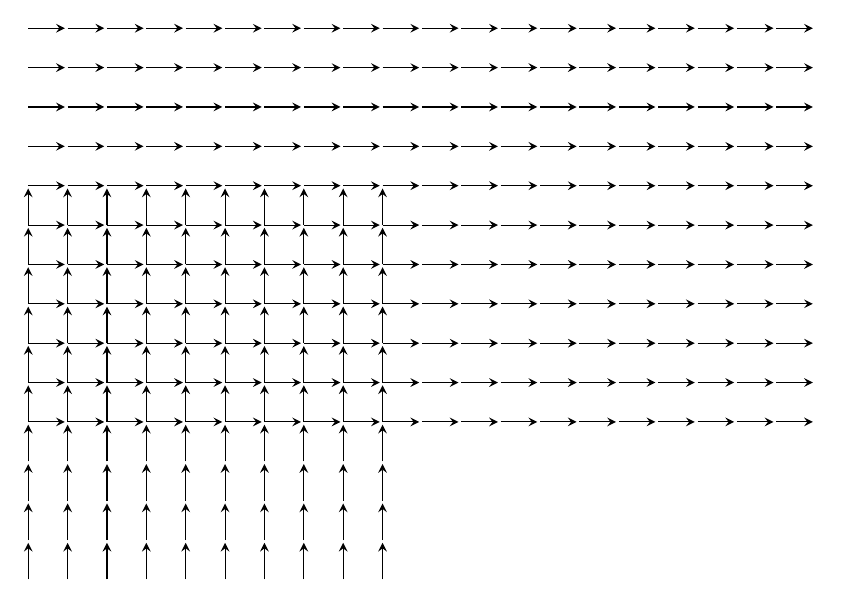
\begin{tikzpicture}[x=0.5cm,y=0.5cm,>=stealth,shorten >=1pt]
\foreach \x in {1,...,10}{
    \foreach \y in {1,...,10}{
	\draw[->] (\x,\y) -- (\x,\y+1);
    }
}
\foreach \x in {1,...,20}{
    \foreach \y in {5,...,15}{
	\draw[->] (\x,\y) -- (\x+1,\y);
    }
}
\end{tikzpicture}
\end{center}
\caption{The relation from \autoref{ex:closure4}}
\label{f:closure4}
\end{figure}
\begin{example}
\label{ex:closure4}
Consider the relation in example {\tt closure4} that comes with
the Omega calculator~\shortcite{Omega_calc}, $R = R_1 \cup R_2$,
with
$$
\begin{aligned}
R_1 & = \{\, (x,y) \to (x,y+1) \mid 1 \le x,y \le 10 \,\}
\\
R_2 & = \{\, (x,y) \to (x+1,y) \mid 1 \le x \le 20 \wedge 5 \le y \le 15 \,\}
.
\end{aligned}
$$
This relation is shown graphically in \autoref{f:closure4}.
We have
$$
\begin{aligned}
R_1 \circ R_2 &=
\{\, (x,y) \to (x+1,y+1) \mid 1 \le x \le 9 \wedge 5 \le y \le 10 \,\}
\\
R_2 \circ R_1 &=
\{\, (x,y) \to (x+1,y+1) \mid 1 \le x \le 10 \wedge 4 \le y \le 10 \,\}
.
\end{aligned}
$$
Clearly, $R_1 \circ R_2 \subseteq R_2 \circ R_1$ and so
$$
\left(
R_1 \cup R_2
\right)^+
=
\left(R_2^+ \circ R_1^+\right)
\cup R_1^+
\cup R_2^+
.
$$
\end{example}

\begin{figure}
\newcounter{n}
\newcounter{t1}
\newcounter{t2}
\newcounter{t3}
\newcounter{t4}
\begin{center}
\begin{tikzpicture}[>=stealth,shorten >=1pt]
\setcounter{n}{7}
\foreach \i in {1,...,\value{n}}{
    \foreach \j in {1,...,\value{n}}{
	\setcounter{t1}{2 * \j - 4 - \i + 1}
	\setcounter{t2}{\value{n} - 3 - \i + 1}
	\setcounter{t3}{2 * \i - 1 - \j + 1}
	\setcounter{t4}{\value{n} - \j + 1}
	\ifnum\value{t1}>0\ifnum\value{t2}>0
	\ifnum\value{t3}>0\ifnum\value{t4}>0
	    \draw[thick,->] (\i,\j) to[out=20] (\i+3,\j);
	\fi\fi\fi\fi
	\setcounter{t1}{2 * \j - 1 - \i + 1}
	\setcounter{t2}{\value{n} - \i + 1}
	\setcounter{t3}{2 * \i - 4 - \j + 1}
	\setcounter{t4}{\value{n} - 3 - \j + 1}
	\ifnum\value{t1}>0\ifnum\value{t2}>0
	\ifnum\value{t3}>0\ifnum\value{t4}>0
	    \draw[thick,->] (\i,\j) to[in=-20,out=20] (\i,\j+3);
	\fi\fi\fi\fi
	\setcounter{t1}{2 * \j - 1 - \i + 1}
	\setcounter{t2}{\value{n} - 1 - \i + 1}
	\setcounter{t3}{2 * \i - 1 - \j + 1}
	\setcounter{t4}{\value{n} - 1 - \j + 1}
	\ifnum\value{t1}>0\ifnum\value{t2}>0
	\ifnum\value{t3}>0\ifnum\value{t4}>0
	    \draw[thick,->] (\i,\j) to (\i+1,\j+1);
	\fi\fi\fi\fi
    }
}
\end{tikzpicture}
\end{center}
\caption{The relation from \autoref{ex:decomposition}}
\label{f:decomposition}
\end{figure}
\begin{example}
\label{ex:decomposition}
Consider the relation on the right of \shortciteN[Figure~2]{Beletska2009},
reproduced in \autoref{f:decomposition}.
The relation can be described as $R = R_1 \cup R_2 \cup R_3$,
with
$$
\begin{aligned}
R_1 &= n \mapsto \{\, (i,j) \to (i+3,j) \mid
i \le 2 j - 4 \wedge
i \le n - 3 \wedge
j \le 2 i - 1 \wedge
j \le n \,\}
\\
R_2 &= n \mapsto \{\, (i,j) \to (i,j+3) \mid
i \le 2 j - 1 \wedge
i \le n \wedge
j \le 2 i - 4 \wedge
j \le n - 3 \,\}
\\
R_3 &= n \mapsto \{\, (i,j) \to (i+1,j+1) \mid
i \le 2 j - 1 \wedge
i \le n - 1 \wedge
j \le 2 i - 1 \wedge
j \le n - 1\,\}
.
\end{aligned}
$$
The figure shows this relation for $n = 7$.
Both
$R_3 \circ R_1 \subseteq R_1 \circ R_3$
and
$R_3 \circ R_2 \subseteq R_2 \circ R_3$,
which the reader can verify using the {\tt iscc} calculator:
\begin{verbatim}
R1 := [n] -> { [i,j] -> [i+3,j] : i <= 2 j - 4 and i <= n - 3 and
                                  j <= 2 i - 1 and j <= n };
R2 := [n] -> { [i,j] -> [i,j+3] : i <= 2 j - 1 and i <= n and
                                  j <= 2 i - 4 and j <= n - 3 };
R3 := [n] -> { [i,j] -> [i+1,j+1] : i <= 2 j - 1 and i <= n - 1 and
                                    j <= 2 i - 1 and j <= n - 1 };
(R1 . R3) - (R3 . R1);
(R2 . R3) - (R3 . R2);
\end{verbatim}
$R_3$ can therefore be moved forward in any path.
For the other two basic relations, we have both
$R_2 \circ R_1 \not\subseteq R_1 \circ R_2$
and
$R_1 \circ R_2 \not\subseteq R_2 \circ R_1$
and so $R_1$ and $R_2$ form a strongly connected component.
By computing the power of $R_3$ and $R_1 \cup R_2$ separately
and composing the results, the power of $R$ can be computed exactly
using \eqref{eq:transitive:singleton}.
As explained by \shortciteN{Beletska2009}, applying the same formula
to $R$ directly, without a decomposition, would result in
an overapproximation of the power.
\end{example}

\subsection{Partitioning the domains and ranges of $R$}

The algorithm of \autoref{s:power} assumes that the input relation $R$
can be treated as a union of translations.
This is a reasonable assumption if $R$ maps elements of a given
abstract domain to the same domain.
However, if $R$ is a union of relations that map between different
domains, then this assumption no longer holds.
In particular, when an entire dependence graph is encoded
in a single relation, as is done by, e.g.,
\shortciteN[Section~6.1]{Barthou2000MSE}, then it does not make
sense to look at differences between iterations of different domains.
Now, arguably, a modified Floyd-Warshall algorithm should
be applied to the dependence graph, as advocated by
\shortciteN{Kelly1996closure}, with the transitive closure operation
only being applied to relations from a given domain to itself.
However, it is also possible to detect disjoint domains and ranges
and to apply Floyd-Warshall internally.

\LinesNumbered
\begin{algorithm}
\caption{The modified Floyd-Warshall algorithm of
\protect\shortciteN{Kelly1996closure}}
\label{a:Floyd}
\SetKwInput{Input}{Input}
\SetKwInput{Output}{Output}
\Input{Relations $R_{pq}$, $0 \le p, q < n$}
\Output{Updated relations $R_{pq}$ such that each relation
$R_{pq}$ contains all indirect paths from $p$ to $q$ in the input graph}
%
\BlankLine
\SetAlgoVlined
\DontPrintSemicolon
%
\For{$r \in [0, n-1]$}{
    $R_{rr} \coloneqq R_{rr}^+$ \nllabel{l:Floyd:closure}\;
    \For{$p \in [0, n-1]$}{
	\For{$q \in [0, n-1]$}{
	    \If{$p \ne r$ or $q \ne r$}{
		$R_{pq} \coloneqq R_{pq} \cup \left(R_{rq} \circ R_{pr}\right)
			     \cup \left(R_{rq} \circ R_{rr} \circ R_{pr}\right)$
	     \nllabel{l:Floyd:update}
	     }
	}
    }
}
\end{algorithm}

Let the input relation $R$ be a union of $m$ basic relations $R_i$.
Let $D_{2i}$ be the domains of $R_i$ and $D_{2i+1}$ the ranges of $R_i$.
The first step is to group overlapping $D_j$ until a partition is
obtained.  If the resulting partition consists of a single part,
then we continue with the algorithm of \autoref{s:power}.
Otherwise, we apply Floyd-Warshall on the graph with as vertices
the parts of the partition and as edges the $R_i$ attached to
the appropriate pairs of vertices.
In particular, let there be $n$ parts $P_k$ in the partition.
We construct $n^2$ relations
$$
R_{pq} \coloneqq \bigcup_{i \text{ s.t. } \domain R_i \subseteq P_p \wedge
				 \range R_i \subseteq P_q} R_i
,
$$
apply \autoref{a:Floyd} and return the union of all resulting
$R_{pq}$ as the transitive closure of $R$.
Each iteration of the $r$-loop in \autoref{a:Floyd} updates
all relations $R_{pq}$ to include paths that go from $p$ to $r$,
possibly stay there for a while, and then go from $r$ to $q$.
Note that paths that ``stay in $r$'' include all paths that
pass through earlier vertices since $R_{rr}$ itself has been updated
accordingly in previous iterations of the outer loop.
In principle, it would be sufficient to use the $R_{pr}$
and $R_{rq}$ computed in the previous iteration of the
$r$-loop in Line~\ref{l:Floyd:update}.
However, from an implementation perspective, it is easier
to allow either or both of these to have been updated
in the same iteration of the $r$-loop.
This may result in duplicate paths, but these can usually
be removed by coalescing (\autoref{s:coalescing}) the result of the union
in Line~\ref{l:Floyd:update}, which should be done in any case.
The transitive closure in Line~\ref{l:Floyd:closure}
is performed using a recursive call.  This recursive call
includes the partitioning step, but the resulting partition will
usually be a singleton.
The result of the recursive call will either be exact or an
overapproximation.  The final result of Floyd-Warshall is therefore
also exact or an overapproximation.

\begin{figure}
\begin{center}
\begin{tikzpicture}[x=1cm,y=1cm,>=stealth,shorten >=3pt]
\foreach \x/\y in {0/0,1/1,3/2} {
    \fill (\x,\y) circle (2pt);
}
\foreach \x/\y in {0/1,2/2,3/3} {
    \draw (\x,\y) circle (2pt);
}
\draw[->] (0,0) -- (0,1);
\draw[->] (0,1) -- (1,1);
\draw[->] (2,2) -- (3,2);
\draw[->] (3,2) -- (3,3);
\draw[->,dashed] (2,2) -- (3,3);
\draw[->,dotted] (0,0) -- (1,1);
\end{tikzpicture}
\end{center}
\caption{The relation (solid arrows) on the right of Figure~1 of
\protect\shortciteN{Beletska2009} and its transitive closure}
\label{f:COCOA:1}
\end{figure}
\begin{example}
Consider the relation on the right of Figure~1 of
\shortciteN{Beletska2009},
reproduced in \autoref{f:COCOA:1}.
This relation can be described as
$$
\begin{aligned}
\{\, (x, y) \to (x_2, y_2) \mid {} & (3y = 2x \wedge x_2 = x \wedge 3y_2 = 3 + 2x \wedge x \ge 0 \wedge x \le 3) \vee {} \\
& (x_2 = 1 + x \wedge y_2 = y \wedge x \ge 0 \wedge 3y \ge 2 + 2x \wedge x \le 2 \wedge 3y \le 3 + 2x) \,\}
.
\end{aligned}
$$
Note that the domain of the upward relation overlaps with the range
of the rightward relation and vice versa, but that the domain
of neither relation overlaps with its own range or the domain of
the other relation.
The domains and ranges can therefore be partitioned into two parts,
$P_0$ and $P_1$, shown as the white and black dots in \autoref{f:COCOA:1},
respectively.
Initially, we have
$$
\begin{aligned}
R_{00} & = \emptyset
\\
R_{01} & = 
\{\, (x, y) \to (x+1, y) \mid 
(x \ge 0 \wedge 3y \ge 2 + 2x \wedge x \le 2 \wedge 3y \le 3 + 2x) \,\}
\\
R_{10} & =
\{\, (x, y) \to (x_2, y_2) \mid (3y = 2x \wedge x_2 = x \wedge 3y_2 = 3 + 2x \wedge x \ge 0 \wedge x \le 3) \,\}
\\
R_{11} & = \emptyset
.
\end{aligned}
$$
In the first iteration, $R_{00}$ remains the same ($\emptyset^+ = \emptyset$).
$R_{01}$ and $R_{10}$ are therefore also unaffected, but
$R_{11}$ is updated to include $R_{01} \circ R_{10}$, i.e.,
the dashed arrow in the figure.
This new $R_{11}$ is obviously transitively closed, so it is not
changed in the second iteration and it does not have an effect
on $R_{01}$ and $R_{10}$.  However, $R_{00}$ is updated to
include $R_{10} \circ R_{01}$, i.e., the dotted arrow in the figure.
The transitive closure of the original relation is then equal to
$R_{00} \cup R_{01} \cup R_{10} \cup R_{11}$.
\end{example}

\subsection{Incremental Computation}
\label{s:incremental}

In some cases it is possible and useful to compute the transitive closure
of union of basic relations incrementally.  In particular,
if $R$ is a union of $m$ basic maps,
$$
R = \bigcup_j R_j
,
$$
then we can pick some $R_i$ and compute the transitive closure of $R$ as
\begin{equation}
\label{eq:transitive:incremental}
R^+ = R_i^+ \cup
\left(
\bigcup_{j \ne i}
R_i^* \circ R_j \circ R_i^*
\right)^+
.
\end{equation}
For this approach to be successful, it is crucial that each
of the disjuncts in the argument of the second transitive
closure in \eqref{eq:transitive:incremental} be representable
as a single basic relation, i.e., without a union.
If this condition holds, then by using \eqref{eq:transitive:incremental},
the number of disjuncts in the argument of the transitive closure
can be reduced by one.
Now, $R_i^* = R_i^+ \cup \identity$, but in some cases it is possible
to relax the constraints of $R_i^+$ to include part of the identity relation,
say on domain $D$.  We will use the notation
${\cal C}(R_i,D) = R_i^+ \cup \identity_D$ to represent
this relaxed version of $R^+$.
\shortciteN{Kelly1996closure} use the notation $R_i^?$.
${\cal C}(R_i,D)$ can be computed by allowing $k$ to attain
the value $0$ in \eqref{eq:transitive:Q} and by using
$$
P \cap \left(D \to D\right)
$$
instead of \eqref{eq:transitive:approx}.
Typically, $D$ will be a strict superset of both $\domain R_i$
and $\range R_i$.  We therefore need to check that domain
and range of the transitive closure are part of ${\cal C}(R_i,D)$,
i.e., the part that results from the paths of positive length ($k \ge 1$),
are equal to the domain and range of $R_i$.
If not, then the incremental approach cannot be applied for
the given choice of $R_i$ and $D$.

In order to be able to replace $R^*$ by ${\cal C}(R_i,D)$
in \eqref{eq:transitive:incremental}, $D$ should be chosen
to include both $\domain R$ and $\range R$, i.e., such
that $\identity_D \circ R_j \circ \identity_D = R_j$ for all $j\ne i$.
\shortciteN{Kelly1996closure} say that they use
$D = \domain R_i \cup \range R_i$, but presumably they mean that
they use $D = \domain R \cup \range R$.
Now, this expression of $D$ contains a union, so it not directly usable.
\shortciteN{Kelly1996closure} do not explain how they avoid this union.
Apparently, in their implementation,
they are using the convex hull of $\domain R \cup \range R$
or at least an approximation of this convex hull.
We use the simple hull (\autoref{s:simple hull}) of $\domain R \cup \range R$.

It is also possible to use a domain $D$ that does {\em not\/}
include $\domain R \cup \range R$, but then we have to
compose with ${\cal C}(R_i,D)$ more selectively.
In particular, if we have
\begin{equation}
\label{eq:transitive:right}
\text{for each $j \ne i$ either }
\domain R_j \subseteq D \text{ or } \domain R_j \cap \range R_i = \emptyset
\end{equation}
and, similarly,
\begin{equation}
\label{eq:transitive:left}
\text{for each $j \ne i$ either }
\range R_j \subseteq D \text{ or } \range R_j \cap \domain R_i = \emptyset
\end{equation}
then we can refine \eqref{eq:transitive:incremental} to
$$
R_i^+ \cup
\left(
\left(
\bigcup_{\shortstack{$\scriptstyle\domain R_j \subseteq D $\\
		     $\scriptstyle\range R_j \subseteq D$}}
{\cal C} \circ R_j \circ {\cal C}
\right)
\cup
\left(
\bigcup_{\shortstack{$\scriptstyle\domain R_j \cap \range R_i = \emptyset$\\
		     $\scriptstyle\range R_j \subseteq D$}}
\!\!\!\!\!
{\cal C} \circ R_j
\right)
\cup
\left(
\bigcup_{\shortstack{$\scriptstyle\domain R_j \subseteq D $\\
		     $\scriptstyle\range R_j \cap \domain R_i = \emptyset$}}
\!\!\!\!\!
R_j \circ {\cal C}
\right)
\cup
\left(
\bigcup_{\shortstack{$\scriptstyle\domain R_j \cap \range R_i = \emptyset$\\
		     $\scriptstyle\range R_j \cap \domain R_i = \emptyset$}}
\!\!\!\!\!
R_j
\right)
\right)^+
.
$$
If only property~\eqref{eq:transitive:right} holds,
we can use
$$
R_i^+ \cup
\left(
\left(
R_i^+ \cup \identity
\right)
\circ
\left(
\left(
\bigcup_{\shortstack{$\scriptstyle\domain R_j \subseteq D $}}
R_j \circ {\cal C}
\right)
\cup
\left(
\bigcup_{\shortstack{$\scriptstyle\domain R_j \cap \range R_i = \emptyset$}}
\!\!\!\!\!
R_j
\right)
\right)^+
\right)
,
$$
while if only property~\eqref{eq:transitive:left} holds,
we can use
$$
R_i^+ \cup
\left(
\left(
\left(
\bigcup_{\shortstack{$\scriptstyle\range R_j \subseteq D $}}
{\cal C} \circ R_j
\right)
\cup
\left(
\bigcup_{\shortstack{$\scriptstyle\range R_j \cap \domain R_i = \emptyset$}}
\!\!\!\!\!
R_j
\right)
\right)^+
\circ
\left(
R_i^+ \cup \identity
\right)
\right)
.
$$

It should be noted that if we want the result of the incremental
approach to be transitively closed, then we can only apply it
if all of the transitive closure operations involved are exact.
If, say, the second transitive closure in \eqref{eq:transitive:incremental}
contains extra elements, then the result does not necessarily contain
the composition of these extra elements with powers of $R_i$.

\subsection{An {\tt Omega}-like implementation}

While the main algorithm of \shortciteN{Kelly1996closure} is
designed to compute and underapproximation of the transitive closure,
the authors mention that they could also compute overapproximations.
In this section, we describe our implementation of an algorithm
that is based on their ideas.
Note that the {\tt Omega} library computes underapproximations
\shortcite[Section 6.4]{Omega_lib}.

The main tool is Equation~(2) of \shortciteN{Kelly1996closure}.
The input relation $R$ is first overapproximated by a ``d-form'' relation
$$
\{\, \vec i \to \vec j \mid \exists \vec \alpha :
\vec L \le \vec j - \vec i \le \vec U
\wedge
(\forall p : j_p - i_p = M_p \alpha_p)
\,\}
,
$$
where $p$ ranges over the dimensions and $\vec L$, $\vec U$ and
$\vec M$ are constant integer vectors.  The elements of $\vec U$
may be $\infty$, meaning that there is no upper bound corresponding
to that element, and similarly for $\vec L$.
Such an overapproximation can be obtained by computing strides,
lower and upper bounds on the difference set $\Delta \, R$.
The transitive closure of such a ``d-form'' relation is
\begin{equation}
\label{eq:omega}
\{\, \vec i \to \vec j \mid \exists \vec \alpha, k :
k \ge 1 \wedge
k \, \vec L \le \vec j - \vec i \le k \, \vec U
\wedge
(\forall p : j_p - i_p = M_p \alpha_p)
\,\}
.
\end{equation}
The domain and range of this transitive closure are then
intersected with those of the input relation.
This is a special case of the algorithm in \autoref{s:power}.

In their algorithm for computing lower bounds, the authors
use the above algorithm as a substep on the disjuncts in the relation.
At the end, they say
\begin{quote}
If an upper bound is required, it can be calculated in a manner
similar to that of a single conjunct [sic] relation.
\end{quote}
Presumably, the authors mean that a ``d-form'' approximation
of the whole input relation should be used.
However, the accuracy can be improved by also trying to
apply the incremental technique from the same paper,
which is explained in more detail in \autoref{s:incremental}.
In this case, ${\cal C}(R_i,D)$ can be obtained by
allowing the value zero for $k$ in \eqref{eq:omega},
i.e., by computing
$$
\{\, \vec i \to \vec j \mid \exists \vec \alpha, k :
k \ge 0 \wedge
k \, \vec L \le \vec j - \vec i \le k \, \vec U
\wedge
(\forall p : j_p - i_p = M_p \alpha_p)
\,\}
.
$$
In our implementation we take as $D$ the simple hull
(\autoref{s:simple hull}) of $\domain R \cup \range R$.
To determine whether it is safe to use ${\cal C}(R_i,D)$,
we check the following conditions, as proposed by
\shortciteN{Kelly1996closure}:
${\cal C}(R_i,D) - R_i^+$ is not a union and for each $j \ne i$
the condition
$$
\left({\cal C}(R_i,D) - R_i^+\right)
\circ
R_j
\circ
\left({\cal C}(R_i,D) - R_i^+\right)
=
R_j
$$
holds.
